\documentclass[11pt]{iopart}
\usepackage[english]{babel}
\pdfoutput=1
%\usepackage{amsmath}
\usepackage{wasysym}
\usepackage{booktabs}
\usepackage{amssymb}
\usepackage{amsbsy}
\usepackage{verbatim}
\usepackage{graphicx}
\usepackage{epstopdf}
\usepackage{color}
\usepackage{sidecap}
\usepackage{bm}% bold math

\usepackage[colorlinks,bookmarks=false,citecolor=blue,linkcolor=red,urlcolor=blue]{hyperref}

%\usepackage{cite}

%
% WARNING !!!!
% 
% iopart.cls definition of \tableofcontents overwrites the
% short title printed every page. 
% The following redefinition of \tableofcontents fixes the
% the problem. 

\catcode`@=11 % If we need private TeX macros
\renewcommand\tableofcontents{%
  \section*{\contentsname}%
  \@starttoc{toc}%
}
\catcode`@=12% '@' is no more a character
\newcommand{\bra}[1]{\langle\left.{#1}\right|}
\newcommand{\ket}[1]{\left|{#1}\right.\rangle}


\def\be{\begin{equation}}
\def\ee{\end{equation}}
\def\u{\uparrow}
\def\d{\downarrow}
\def\nm{\newmoon}
\def\fm{\fullmoon}
\def\T{\rule{0pt}{.6cm}}
\def\B{\rule[-.4cm]{0pt}{0pt}}

\begin{document}

\setlength{\parindent}{0pt}


\title{Finite-size study of the Quench Action approach in integrable spin 
chains}

\author{Vincenzo Alba$^1$, Pasquale Calabrese$^1$}
\address{$^1$ International School for Advanced Studies (SISSA),
Via Bonomea 265, 34136, Trieste, Italy,
INFN, Sezione di Trieste}


\date{\today}



%%%%%%%%%%%%%%%%%%%%%%%%%%%%%%%%%%%%%%%%%%%%%%%%%%%%%%%%%%%%%%%%%%%%%%%%%%
\begin{abstract} 


fdasfa
\end{abstract}

\maketitle

%%%%%%%%%%%%%%%%% INTRODUCTION %%%%%%%%%%%%%%%%%%%%%
\section{Introduction}
\label{intro}

%%%%%% NEEL OVERLAP
\section{Overlap with the Neel state}

Let us consider a generic $n$-string state
%
\begin{equation}
\lambda_{n;\alpha}^{a}=\lambda_{n;\alpha}+\frac{i}{2}(n+1-2a)+i\delta_{n;\alpha}^{a}
\quad\textrm{with}\, a=1,\dots, n.
\end{equation}
%
We denote the generic parity invariant eigenstate as $|\{\pm\lambda_j\}_{j=1}^m,n_\infty\rangle$, 
where $m$ is the number of rapidity pairs, $N_{\infty}$ is the number of infinite rapidities, 
with $M=L/2=N_\infty+2m$, and $n_\infty\equiv N_\infty/L$ is the infinite rapidities density. 

The overlap with the Neel state $|\Psi_0\rangle$ reads 
%
\begin{equation}
\label{neel-ov}
\frac{\langle\Psi_0|\{\pm\lambda_j\}_{j=1}^m,n_\infty\rangle}{|||\{\lambda_j\}_{j=1}^m,n_\infty\rangle||}=
\frac{\sqrt{2}N_{\infty}!}{\sqrt{(2N_\infty)!}}\left[\prod_{j=1}^m\frac{\sqrt{\lambda_j^2+1/4}}{4\lambda_j}
\right]\sqrt{\frac{\textrm{det}_m(G^+)}{\textrm{det}_m(G^-)}}
\end{equation}
%
where 
%
\begin{equation}
\label{G-pm}
G^{\pm}_{jk}=\delta_{jk}\left(NK_{1/2}(\lambda_j)-\sum\limits_{l=1}^mK_1^+(\lambda_j,\lambda_l)\right)
+K_{1}^{\pm}(\lambda_j,\lambda_k),\quad\,j,k=1,\dots,m
\end{equation}
%
and 
%
\begin{equation}
\label{K-1}
K_1^\pm(\lambda,\mu)=K_1(\lambda-\mu)\pm K_1(\lambda+\mu)
\end{equation}
%
and 
%
\begin{equation}
\label{K-alpha}
K_\alpha(\lambda)\equiv\frac{2\alpha}{\lambda^2+\alpha^2}
\end{equation}
%

%%%%%% REDUCED NEEL OVERLAP
\subsection{Reduced Neel overlap}

In the case of perfect strings the matrices $G^{\pm}_{jk}$ become ill-defined. Precisely, 
$K_{1}^+(\lambda,\mu)$ diverges if $\lambda$ and $\mu$ are successive members of 
the same string, i.e., $|\lambda-\mu|=i$.  

It is possible to rewrite~\eref{neel-ov} in terms of the string centers $\lambda_{n;\alpha}$ only. 
Here we restrict ourselves to rapidity configurations with no zero-momentum strings. 


It is convenient to split the indices $i,j$ of $G^\pm_{ij}$ as $i=(n,\alpha)$ $j=(m,\beta)$, 
with $n,m$ being the length of the strings and $\alpha,\beta$ labelling the string centers. 

The result reads 
%
\begin{equation}
\fl \frac{1}{2}G^+_{(n,\alpha)(m,\beta)}=\left\{\begin{array}{cc}
L\theta_n'(\lambda_{n;\alpha})
-\sum\limits_{(\ell,\gamma)\ne(n,\alpha)}(\Theta'_{n,\ell}
(\lambda_{n;\alpha}-\lambda_{\ell;\gamma})+\Theta'_{n,\ell}
(\lambda_{n;\alpha}+\lambda_{\ell;\gamma})) & \textrm{if}\,(n,\alpha)= (m,\beta)\\
\Theta'_{n,m}
(\lambda_{n;\alpha}-\lambda_{m;\beta})+\Theta'_{n,m}
(\lambda_{n;\alpha}+\lambda_{m;\beta}) & \textrm{if}\,(n,\alpha)\ne(m,\beta)
\end{array}\right.
\end{equation}
%
Here $\theta_n'(x)\equiv d/dx\theta_n(x)$ and $\Theta'(x)\equiv d/dx\Theta(x)$. 

For $G^-_{ij}$ one obtains 

\begin{equation}
\fl\frac{1}{2}G^-_{(n,\alpha)(m,\beta)}=\left\{\begin{array}{cc}
(L-1)\theta'_n(\lambda_{n;\alpha})-2\sum\limits_{k=1}^{n-1}\theta'_k(\lambda_{n;\alpha})
-\sum\limits_{(\ell,\gamma)\ne(n,\alpha)}(\Theta'_{n,\ell}
(\lambda_{n;\alpha}-\lambda_{\ell;\gamma})+\Theta'_{n,l}
(\lambda_{n;\alpha}+\lambda_{\ell;\gamma})) & \quad\textrm{if}\,(n,\alpha)= (m,\beta)\\
\Theta'_{n,m}
(\lambda_{n;\alpha}-\lambda_{m;\beta})-\Theta'_{n,m}
(\lambda_{n;\alpha}+\lambda_{m;\beta})) & \quad\textrm{if}\,(n,\alpha)\ne(m,\beta)
\end{array}\right.
\end{equation}
%
Finally, the multiplicative prefactor in~\eref{neel-ov} for the generic $n$-string 
can be rewritten as 
%
\begin{equation}
\prod\limits_{a=1}^n\frac{\sqrt{(\lambda^a_{n;\alpha})^2+1/4}}{4\lambda^a_{n;\alpha}}=
\frac{1}{4^n}\left(\frac{\sqrt{n^2+\lambda^2_{n;\alpha}}}{\lambda_{n;\alpha}}
\prod\limits_{k=0}^{\lceil n/2\rceil-1}\frac{(2k)^2+\lambda^2_{n;\alpha}}{(2k+1)^2+
\lambda^2_{n;\alpha}}\right)^{{\mathcal P}},
\end{equation}
%
with ${\mathcal P}=+$ and ${\mathcal P}=-$ for even and odd strings, respectively. 

\begin{table}[h]
\scriptsize
\centering
Bethe states with nonzero N\'eel overlap ($N=12$)\\[1ex]
\begin{tabular}{rrrrr}
String content & $2I^+_n$ & E & $|\langle \{\lambda\}| \Psi_0 \rangle|^2$ & here \\[0.3em]
\toprule
6 inf & - & $0$ & $0.002164502165$ & $0.002164502165$ \\
\midrule
2 one, 4 inf &$1_1 $ & $-3.918985947229$ & $0.096183409244$ & $0.096183409244237$ \\
 &$3_1 $ & $-3.309721467891$ & $0.011288497947$ &  $0.0112884979464673$\\
 &$5_1 $ & $-2.284629676547$ & $0.004542580506$ &  $0.0045425805061850$\\
 &$7_1 $ & $-1.169169973996$ & $0.002752622983$ &  $0.0027526229835876$\\
 &$9_1 $ & $-0.317492934338$ & $0.002116006203$ &  $0.0021160062026402$\\
\midrule
4 one, 2 inf &$1_1 3_1 $ & $-7.070529325964$ & $0.310133033838$ &$ 0.554809782804$ \\
  &$1_1 5_1 $ & $-5.847128730477$ & $0.129277023687$ \\
  &$ 1_1 7_1$ & $-4.570746557876$ & $0.085992436024$ \\
  &$ 3_1 5_1$ & $-5.153853093221$ & $0.015256395523$ \\
  &$3_1 7_1 $ & $-3.916336243695$ & $0.010091113504$ \\
  &$5_1 7_1 $ & $-2.817696043731$ & $0.004059780228$ \\
  \midrule
2 two, 2 inf &$1_2 $ & $-1.905667167442$ & $0.001207238321$ & $0.005468702625$\\
  &$3_2 $ & $-1.368837200825$ & $0.002340453815$ \\
  &$5_2 $ & $-0.681173793635$ & $0.001921010489$ \\
    \midrule
1 one, 1 three, 2 inf &$0_1 0_3 $ & $-2.668031843135$ & $0.034959609810$ & $0.034959609810$ \\
    \midrule
6 one &$1_1 3_1 5_1 $ & $-8.387390917445$ & $0.153412152966$ & $0.153412152966$ \\
  \midrule
2 two, 2 one &$1_1 1_2 $ & $-5.401838225870$ & $0.040162686361$ & $0.046134750850$ \\
  &$3_1 1_2 $ & $-4.613929948329$ & $0.004636541934$ \\
  &$5_1 1_2 $ & $-3.147465758841$ & $0.001335522556$ \\
    \midrule
1 three, 3 one &$0_1 2_1 0_3$ & $-6.340207488736$ & $0.052743525774$ & $0.078910020729$ \\
  &$0_1 4_1 0_3$ & $-5.203653009936$ & $0.015022005621$ \\
  &$0_1 6_1 0_3$ & $-3.788693957250$ & $0.011144489334$ \\
      \midrule
1 five, 1 one &$0_1 0_5$ & $-2.444293750583$ & $0.005887902992$ & $0.005887902992$ \\
      \midrule
2 three &$1_3$ & $-1.111855930538$ & $0.001342476001$ & $0.001342476001$ \\
      \midrule
1 two, 1 four &$0_2 0_4$ & $-1.560671012472$ & $0.000026982174$ & $0.000026982174$ \\
  \bottomrule
 \end{tabular}
\caption{All Bethe states for $N=12$ with nonzero overlap with the zero-momentum N\'eel state. The 
overlap squares add up to $1$ up to the precision in which the Bethe equations were solved. The 
$2I^+_n$ in the second column give the positive $n$-string quantum numbers of the parity-invariant 
Bethe states.}
\label{table:RV:sumruleN12}
\end{table}





%##################################################################
\begin{figure}[t]
\begin{center}
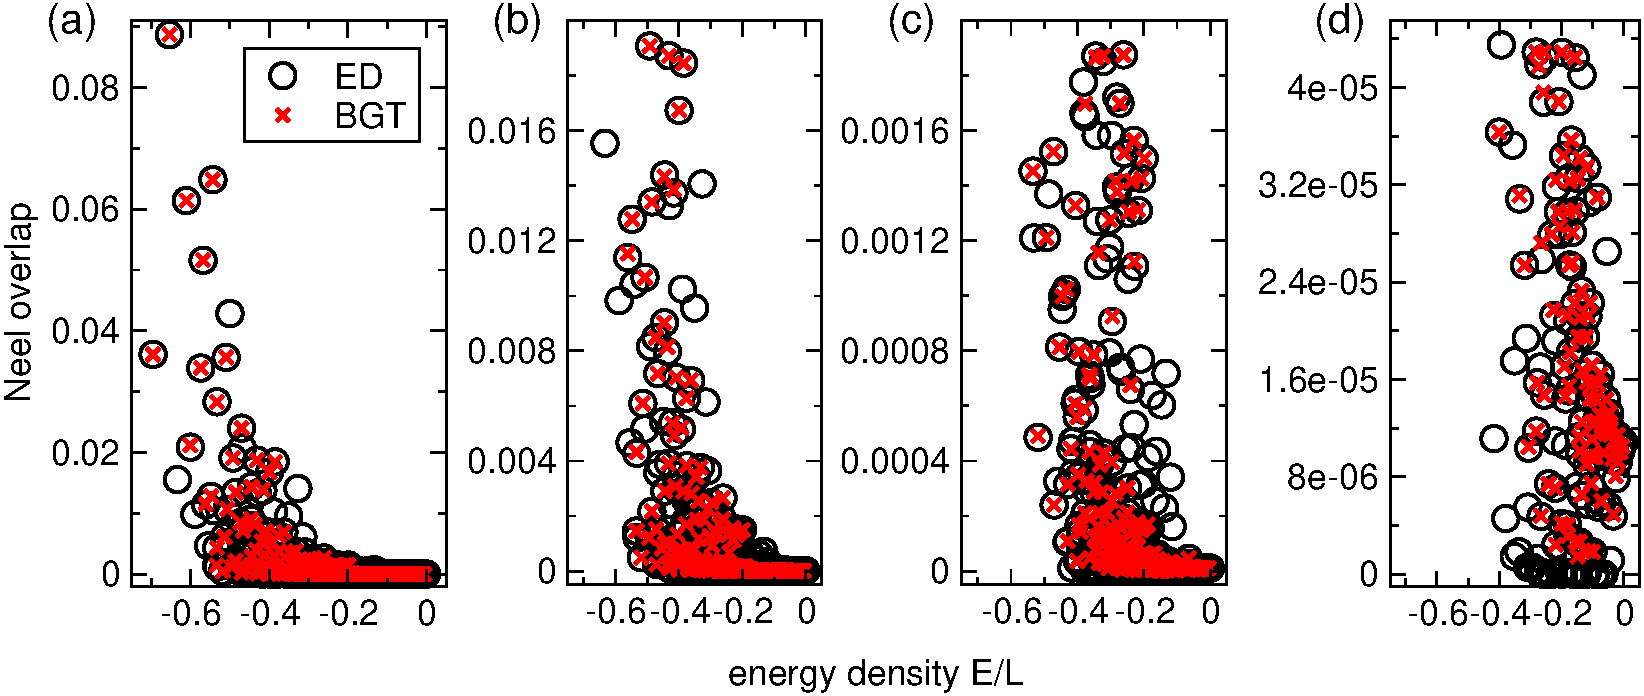
\includegraphics[width=.9\textwidth]{./draft_figs/L20_BT_check}
\end{center}
\caption{ The squared overlap $|\langle\Psi_0|\{\lambda\}\rangle|^2$ between the the 
 Neel state $|\Psi_0\rangle$ and the eigenstates $|\{\lambda\}\rangle$ of the $XXX$ 
 chain with $L=22$ sites. Only non-zero overlaps are shown. In all the panels the 
 $x$-axis shows the eigenstate energy density $E/L$. The circles are the exact 
 diagonalization results for all the non-zero overlaps. The crosses are the Bethe 
 ansatz results obtained using the Bethe-Gaudin-Takahashi equations. The missing 
 crosses correspond to eigenstates containing zero-momentum strings. (a) Overview 
 of all the non-zero overlaps. (b)(c)(d) The same overlaps as in (a) zooming in 
 the regions $[0,0.2]$, $[0,0.020]$, and $[0,4\cdot 10^{-5}]$. The discrepancies 
 between the ED and the Bethe ansatz results are attributed to the string deviations. 
}
\label{fig1-BGT-check}
\end{figure}
%##################################################################


%##################################################################
\begin{figure}[t]
\begin{center}
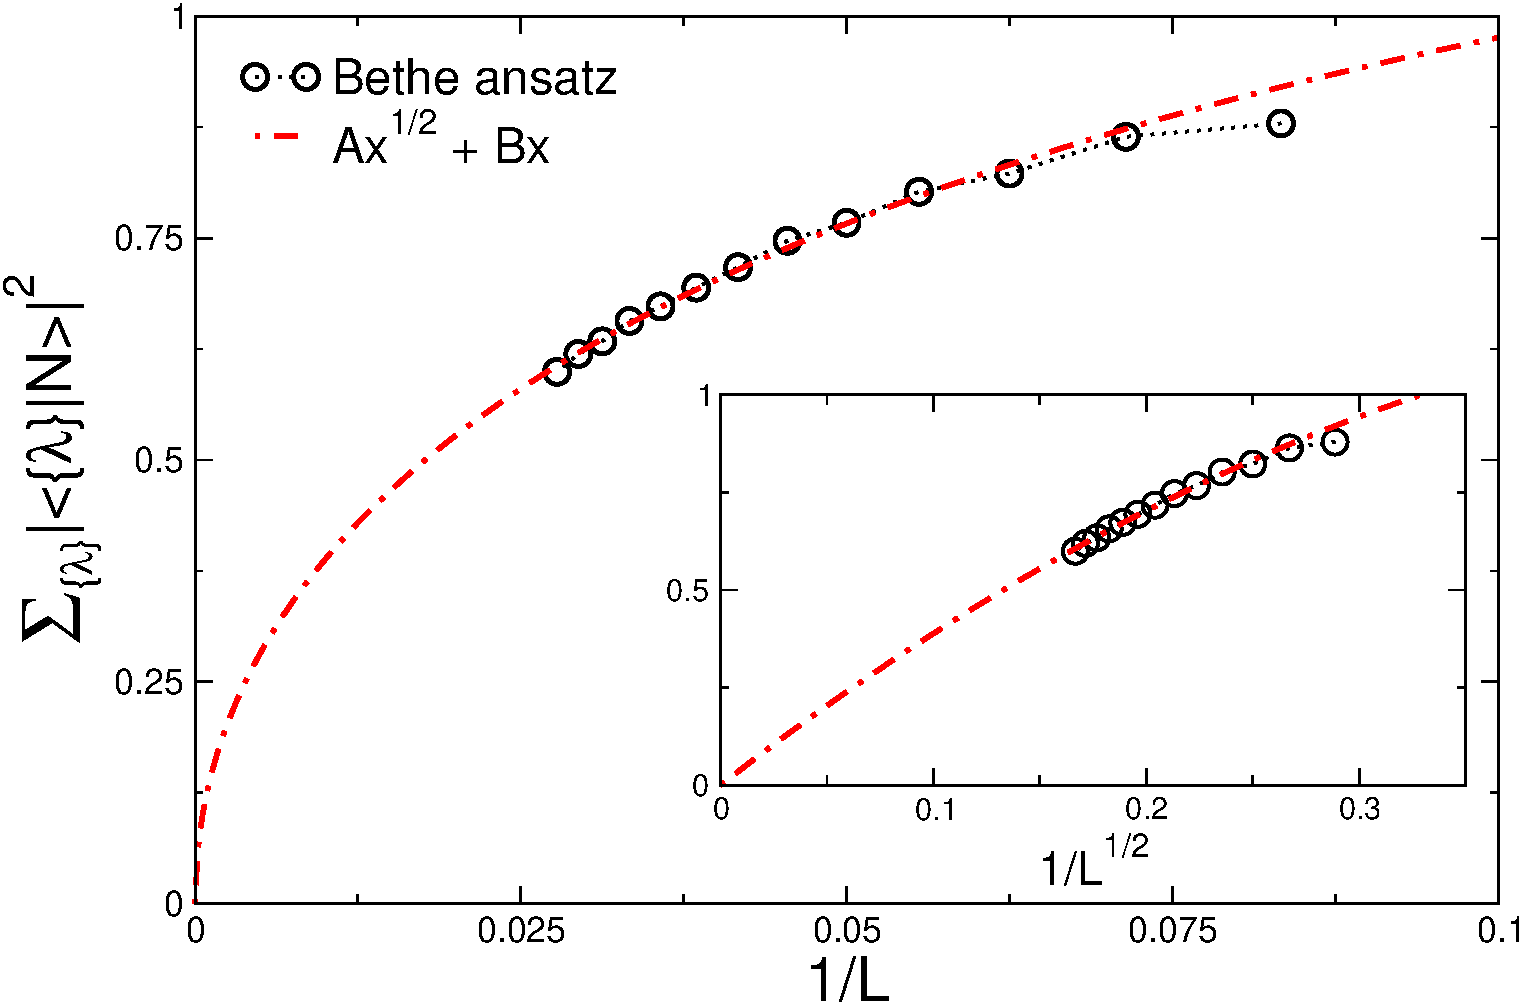
\includegraphics[width=.6\textwidth]{./draft_figs/Neel_over}
\end{center}
\caption{ The overlap sum rule $\sum_{\{\lambda\}}|\langle\{\lambda\}|\Psi_0\rangle|^2$, 
 with $|\Psi_0\rangle$ the Neel state and $|\{\lambda\}\rangle$ the eigenstates  of the 
 $XXX$ spin chain, plotted versus $1/L$, with $L$ the chain length. The circles are 
 Bethe ansatz results for chains up to $L=36$. Only the eigenstates with no zero-momentum 
 strings are considered in the sum. The dash-dotted line is a fit to $A/L^{1/2}+B/L$, with 
 $A,B$ fitting parameters. Inset: The same data as in the main Figure plotted versus 
 $1/L^{1/2}$.
}
\label{fig2-neel-sr}
\end{figure}
%##################################################################


%##################################################################
\begin{figure}[t]
\begin{center}
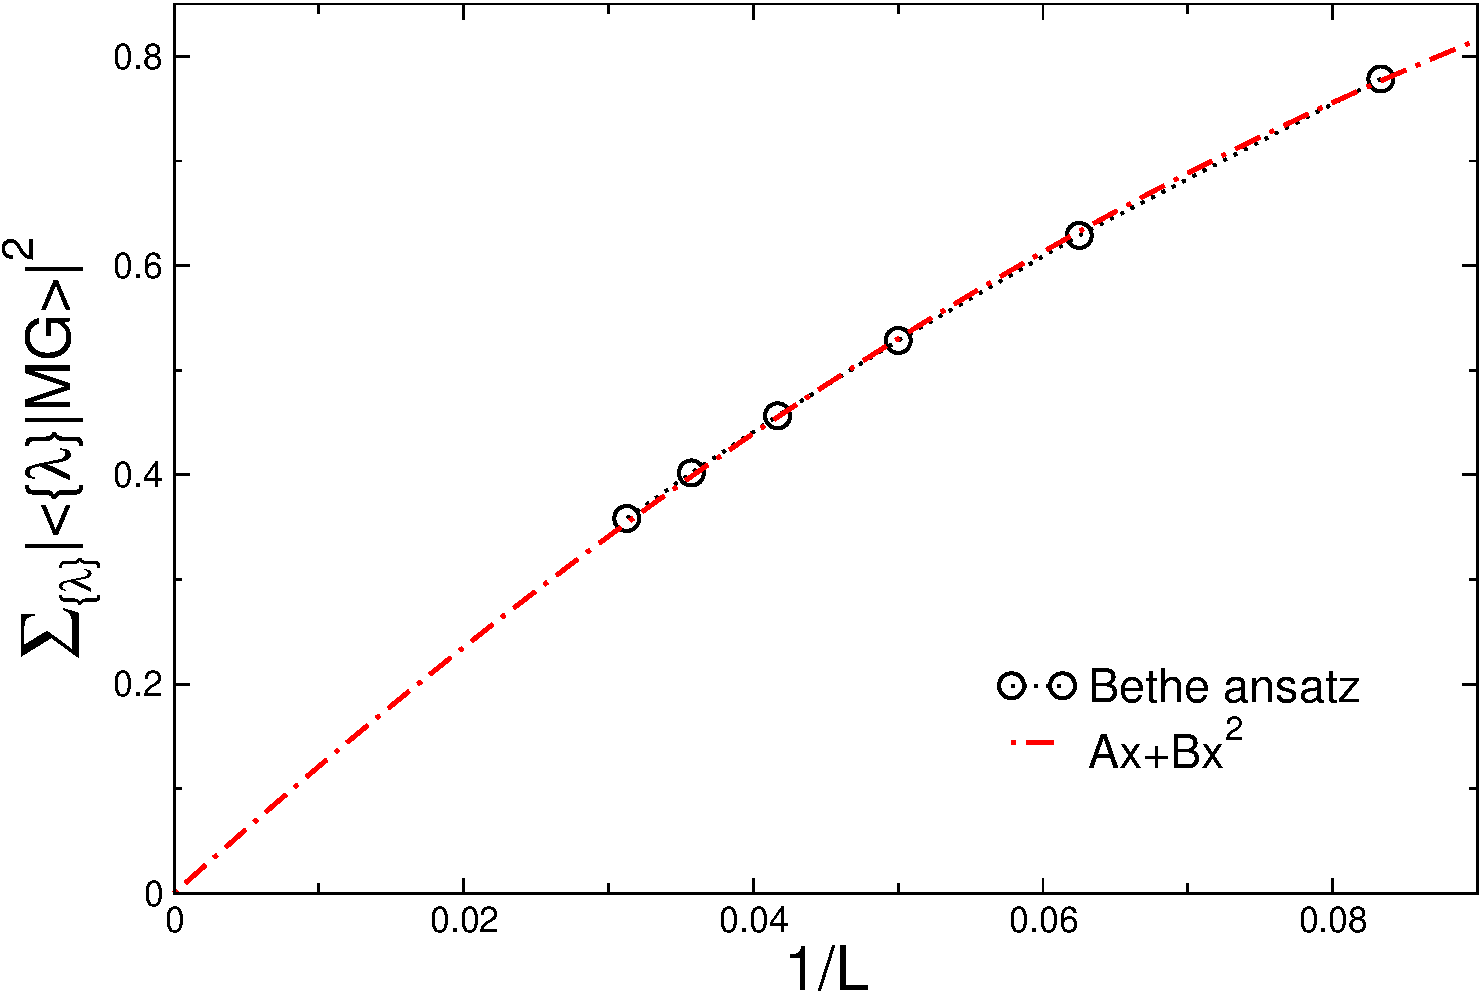
\includegraphics[width=.6\textwidth]{./draft_figs/Dimer_over}
\end{center}
\caption{ The overlap sum rule $\sum_{\{\lambda\}}|\langle\{\lambda\}|\Psi_0\rangle|^2$, 
 with $|\Psi_0\rangle$ the Majumdar-Ghosh state and $|\{\lambda\}\rangle$ the eigenstates  
 of the $XXX$ spin chain, plotted versus $1/L$, with $L$ the chain length. The circles are 
 Bethe ansatz results for chains up to $L=32$. Only the eigenstates with no zero-momentum 
 strings are considered in the sum. The dash-dotted line is a fit to $A/L^{1/2}+B/L$, with 
 $A,B$ fitting parameters. Inset: The same data as in the main Figure plotted versus 
 $1/L^{1/2}$.
}
\label{fig3-dimer-sr}
\end{figure}
%##################################################################


%##################################################################
\begin{figure}[t]
\begin{center}
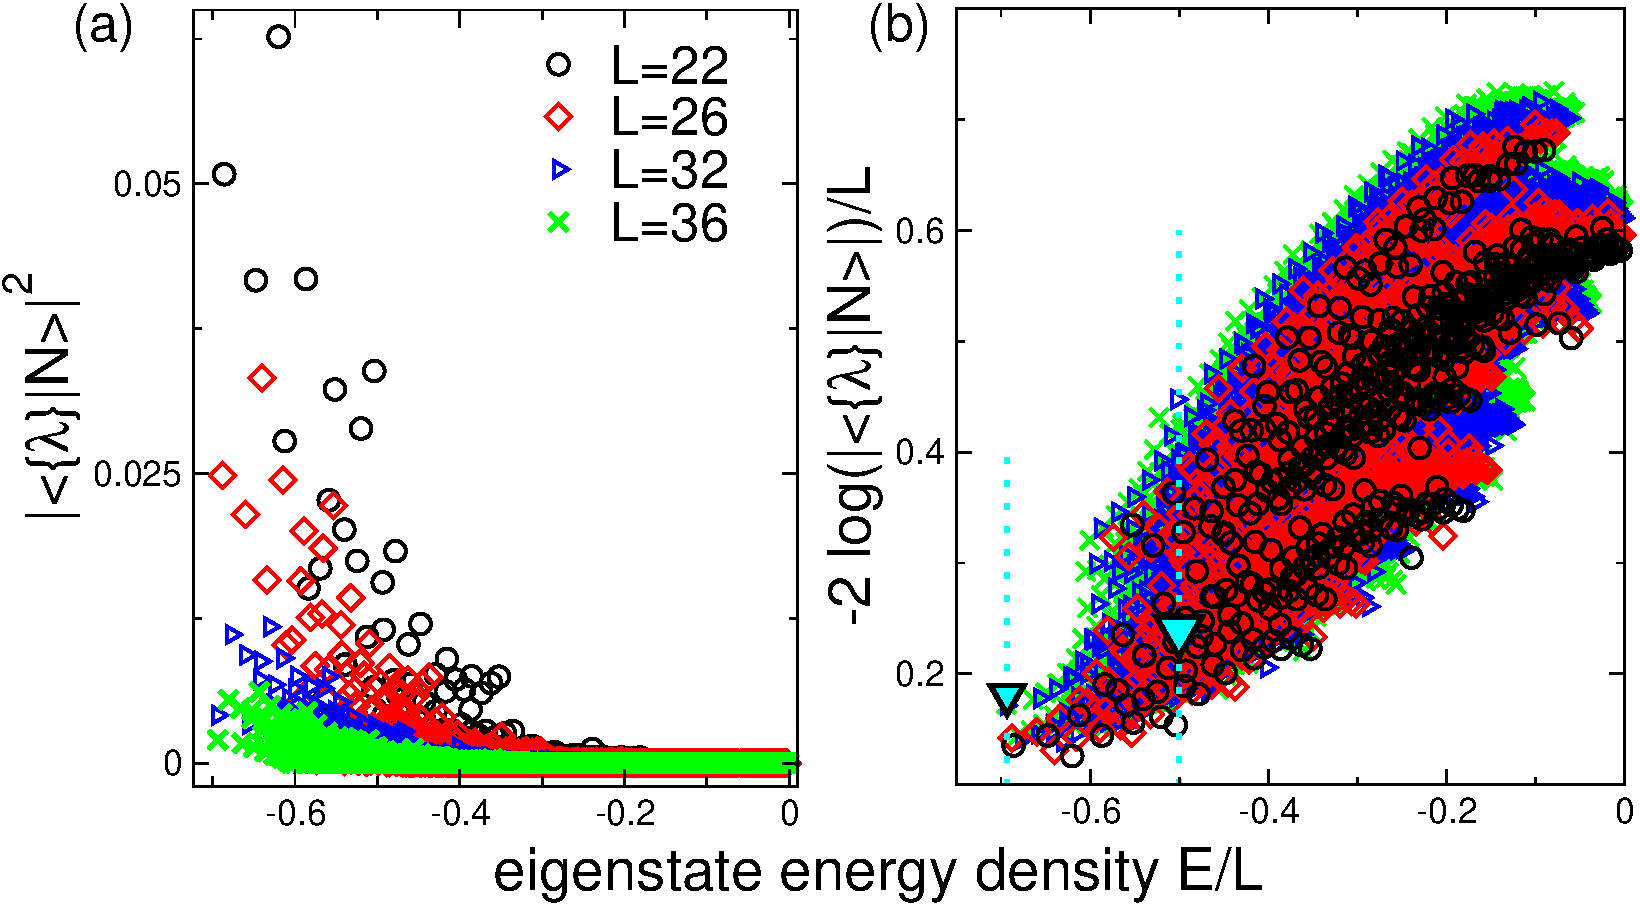
\includegraphics[width=.75\textwidth]{./draft_figs/Neel_over_ener}
\end{center}
\caption{ The overlap between the Neel state and the eigenstates of the 
 $XXX$ chain as a function of the eigenstate energy. (a) The squared 
 overlap $|\langle\{\lambda\}|Neel\rangle|^2$ plotted versus the 
 eigenstates energy density $E/L$. The data are Bethe ansatz results 
 for chains of length $L=22,26,32,36$ (different symbols). (b) Same as 
 in (a) plotting on the $y$-axis the combination $-2\log(|\langle\{
 \lambda\}|Neel\rangle|)/L$. 
}
\label{fig4-neel-ener}
\end{figure}
%##################################################################


%%%%%%%%%%%%%%%%%%%%%% REFERENCES %%%%%%%%%%%%%%%%%%%%%%%%%%%%%%%%%%%%%%%%%%%%%%%%

%\begin{thebibliography}{99}


%\end{thebibliography}


\end{document}


